\chapter{采用线性误差模型的可伸缩视频码流截取}

\section{引言}

能够调整数据源的码率是流媒体系统码率自适应的前提条件。对于SVC视频而言,这意味着从整个码流中截取出一部分数据包。如何在给定的码率下使得截取的失真最小,是码流截取问题的关键。在本章中,我们提出一个线性误差模型和一个基于贪心思想的优先级赋值算法来解决这个问题。

\section{线性误差模型}

\subsection{模型推导}

在H.264/AVC中,解码过程具有线性性质。在不考虑舍入、截断和去块滤波的情况下,解码的主要步骤,如预测、变换、量化等,都可以近似认为是线性操作。基于此,整个解码过程可以用矩阵的形式描述如下:
\begin{equation}
\label{eq:linear}
s = {\rm\bf M} \cdot s + {\rm\bf T} \cdot c + p \: 。
\end{equation}

该式子意味着,一个图像组(GOP)的重建像素, $s$,可以看作如下这三部分的线性组合:该GOP的已重建像素、残差、静态预测子。在公式\ref{eq:linear}中,$c$指代变换系数,$p$是所谓静态预测子;$\rm\bf M$和$\rm\bf T$都是方阵,${\rm\bf M} \cdot s$得到的结果是运动校正预测信号,${\rm\bf T} \cdot c$得到的结果是残差。$\rm\bf M$的实际值由所选择的宏块类型、参考帧索引和运动向量决定,而$\rm\bf T$的实际值取决于所选的量化参数(QP)。

将上述线性解码模型运用到SVC的质量可伸缩中,可以得到一个线性误差模型(LEM)。根据公式\ref{eq:linear},对于一个只包含基本层的码流,有:
\begin{equation}
\label{eq:base0}
s_{B} = {\rm\bf M} \cdot s_{B} + {\rm\bf T}_{B} \cdot c_{B} + p \: ,
\end{equation}
其中带下标$B$的表示是基本层变量。在质量可伸缩中,增强层主要是变换系数的精细化。因此,若一个增强层的数据包集合记为$I_1$,则含有该增强层的码流解码时重建关系可表示为:
\begin{equation}
\label{eq:subset1}
s_{I_1} = {\rm\bf M} \cdot s_{I_1} + {\rm\bf T}_{B} \cdot c_{B} + \Big( \sum_{i \in I_1}{\rm\bf T}_i \cdot c_i \Big) + p \: ,
\end{equation}
其中$i$表示集合$I_1$中的一个增强数据包;$c_i$是一个向量,含有增强层数据包$i$中的变换系数;${\rm\bf T}_i$是由$i$的QP值所决定的变换矩阵,而${\rm\bf T}_i \cdot c_i$得到的就是从$i$解码出来的残差值。

同样的,对于一个含有增强层数据包集合$I_2$的码流,有:
\begin{equation}
\label{eq:subset2}
s_{I_2} = {\rm\bf M} \cdot s_{I_2} + {\rm\bf T}_{B} \cdot c_{B} + \Big( \sum_{i \in I_2}{\rm\bf T}_i \cdot c_i \Big) + p \: 。
\end{equation}

如果$I_1$是$I_2$的子集,那么二者的重建误差就可以由 (\ref{eq:subset2}) - (\ref{eq:subset1})得到:
\begin{equation}
\label{eq:minus1}
(s_{I_2} - s_{I_1}) = {\rm\bf M} \cdot (s_{I_2} - s_{I_1}) + \Big( \sum_{i \in I_2}{\rm\bf T}_i \cdot c_i - \sum_{i \in I_1}{\rm\bf T}_i \cdot c_i \Big) \: ,
\end{equation}
\begin{equation}
\label{eq:minus2}
\Rightarrow e = s_{I_2} - s_{I_1} = ({\rm\bf I - M})^{-1} \cdot \Big( \sum_{i \in I_2}{\rm\bf T}_i \cdot c_i - \sum_{i \in I_1}{\rm\bf T}_i \cdot c_i \Big) \: 。
\end{equation}

特别地,如果$I_2$和$I_1$的差别只有一个增强层数据包$j$,也就是说$I_2 \setminus I_1 = \{j\}$,那么根据(\ref{eq:minus2}),这两个重建序列的差为:
\begin{equation}
\label{eq:error_j}
e_j = ({\rm\bf I - M})^{-1} \cdot {\rm\bf T}_j \cdot c_j \: 。
\end{equation}

可以看到,$e_j$只由数据包$j$决定,与其他的增强层数据包无关。这个值$e_j$被定义为数据包$j$的“误差向量”,表示丢弃数据包$j$后所带来的像素值误差。我们可以通过如下的方式得到任何一个数据包$j$的误差向量:选取两个只差$j$的数据包子集,将它们解码得到的视频序列相减即可。

一旦获取了所有增强层数据包对应的误差向量,那么丢弃任意一个增强层数据包子集所导致的失真就可以用这个子集中的数据包的误差向量之和来估计。举例来说,如果增强层数据包$x$, $y$, $z$从一个码流中被丢弃,那么丢弃前后的重建序列之差应该为:$e = e_x + e_y + e_z$。这个简单的相加之所以合理有两方面的原因。第一,不像MSE或PSNR,误差向量仅仅是像素的差值,并不涉及二次方运算。第二,每个增强层数据包在重建中会各自对像素进行精细化,其效果是叠加的(参见前面的推导过程)。

应该指出,上述第二点原因的成立是有条件的。在公式\ref{eq:base0}-\ref{eq:subset2}中,${\rm\bf M}$和$p$的值都相同是因为,在质量可伸缩的情况下,增强层数据包仅仅是通过操作变换系数得到的,并不涉及运动校正和静态预测过程。然而这对于其他维度的可伸缩(例如视频分辨率改变的空间可伸缩)并不正确。因此,此处推导的线性误差模型并不适用于任意配置的可伸缩视频编码。在本文的研究中,只用到了质量可伸缩;其他伸缩维度将作为未来工作中的探索对象。

\subsection{误差向量获取}

如果按照上一小节中所说,每次计算一个数据包的误差向量,那么所需的解码次数将是所有数据包的个数。这么做的计算量太大。在本小节中,我们给出一个高效获取所有误差向量的方法。

\begin{figure}[h]
\centering
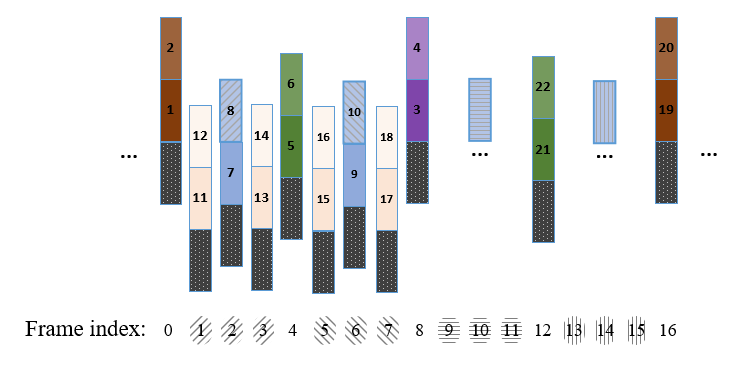
\includegraphics[width = 0.9\linewidth]{figures/GOP-Structure.png}
\caption{SVC码流中的图像组(GOP) \label{fig:GOP_Structure}}
\end{figure}

为了减少解码次数,我们将所有的增强层数据包分成若干组,使得每一组中的多个误差向量能在一次解码中同时获取。考虑如图\ref{fig:GOP_Structure}所示具有8帧图像组结构的一个视频码流。在该图中,基本层数据包是黑色的,增强层数据包按照颜色分为了几个组(相同颜色的属于同一组)。在每一组中,增强层数据包的误差向量可以同时计算,因为这些数据包所影响的像素是互不干扰的。例如,丢弃8号数据包只会在帧1、2、3中带来像素误差,而丢弃10号数据包只会在帧5、6、7中带来像素误差(帧的编号从0开始)。因此,我们可以只通过一次相减来同时得到8号和10号数据包的误差向量$e_{8}$和$e_{10}$,以及所有其他GOP中的相同位置数据包(用相同颜色表示它们属于同一组)的误差向量。应该指出,这些误差向量是非常稀疏的,因为丢弃单个数据包带来的失真影响非常有限。

为了获取所有的误差向量,所需的解码次数大约等于增强层的层数$(L_Q - 1)$乘以时间层的层数$L_T$。对于图\ref{fig:GOP_Structure}中的例子而言,$L_Q = 3$,$L_T = 4$,所以所需的解码次数照此计算将会是$(3 - 1) \times 4 = 8$。然而,我们还需要额外的$L_Q - 1 = 2$次解码,来分离“关键帧”\supercite{H264Overview}(图\ref{fig:GOP_Structure}中的帧0、8、16)中数据包的失真影响。关键帧中增强层数据包的丢弃将会给它两边相邻的两个GOP都带来失真。例如,丢弃4号数据包带来的失真影响范围将会从帧1直到帧15,从而与帧0和帧16中的数据包的失真影响互相交叠。因此,关键帧同一位置的增强层数据包(2、4、20号数据包)应该被分为两个组:一组包含偶数GOP的关键帧数据包(2和20号包),另一组包含奇数GOP的(4号包)。于是,误差向量获取真正所需要的解码次数应为$(L_Q - 1) \cdot (L_T + 1)$。这与JSVM中Quality Layer信息的获取所需的解码次数大致相当。

\subsection{模型验证}

\section{数据包优先级赋值}

\subsection{优先级度量标准}

\subsection{贪心法赋值}

\subsection{无参考源的情况}

\section{实验结果}

\section{本章小结}